\documentclass[12pt]{article}
\usepackage[francais]{babel}
\usepackage[utf8]{inputenc}  
\usepackage{listings}
\usepackage{graphicx}
\usepackage{color}
\usepackage{float}
\usepackage{amsmath}
\usepackage{array}
\usepackage{colortbl}
\usepackage[dvipsnames]{xcolor}
\usepackage{geometry}
\geometry{hmargin=3.5cm,vmargin=3.5cm}

\title{Le jeu de la vie en parralèle}
\author{Benjamin \bsc{Angelaud} - Adrien \bsc{Guilbaud}}
\begin{document}
\maketitle

\section{Introduction}
\paragraph{}Le but de ce TDP est d'implémenter un jeu de la vie avec différentes approches. Dans un premier temps nous partirons de la version séquentielle pour obtenir une version openmp. Ensuite, il sera demandé une version pthread puis 3 versions mpi en changeant de méthode de communication entre les process mpi.

\paragraph{}Tous les tests ont été effectués sur Plafrim. Le schéma de tests par défaut sera de 500 itérations et respectivement des tailles de grille de côté 10, 100, 500, 2000, 8000.

\begin{figure}[!h]
	\begin{center}
		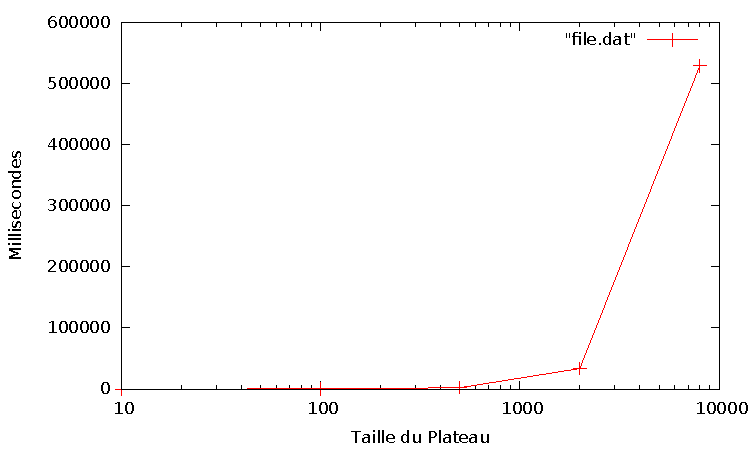
\includegraphics[scale=0.5]{seq.pdf}
	\end{center}
	\caption{Exécution séquentielle \label{fig:life_seq}}
\end{figure} 

\section{Version mémoire partagée}
\subsection{OpenMP}
\paragraph{}Le travail des threads étant relativement uniforme, nous pouvons garder un ordannecement static.
\paragraph{}Ici le but est tout simplement d'ajouter les clauses openmp sur les deux boucles principales qui permettent de compter le nombre de voisins de chaque cellule puis sur la boucle permettant de calculer si une cellule est vivante ou non à la fin de l'étape. On voit donc une optimisation assez conséquente dans le temps d'exécution obtenue assez facilement. A noter que nous avons utiliser 8 threads.

\begin{figure}[!h]
	\begin{center}
		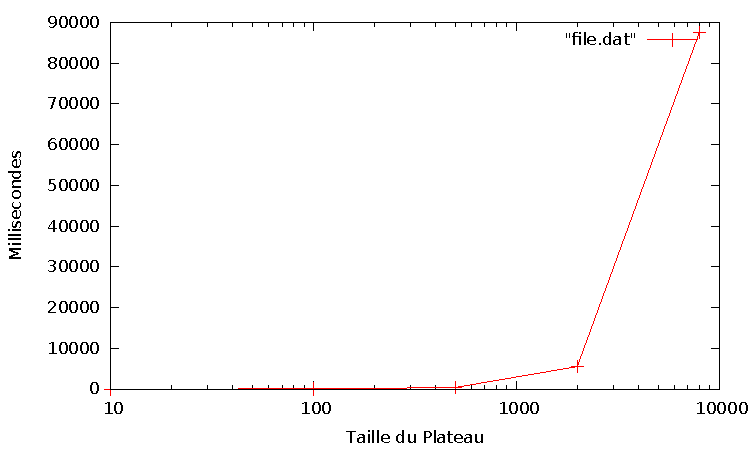
\includegraphics[scale=0.5]{omp.pdf}
	\end{center}
	\caption{Exécution OpenMP \label{fig:life_omp}}
\end{figure}
\subsection{pthread}
\paragraph{} Ici, au début de chaque itération, les cellules dites "fantômes" sont mises à jour. Chaque thread détient une colonne de la grille et va dans un premier temps calculer le nombre de voisins des cellules sur les bords, avant de calculer les voisins des cellules intérieurs. Suite à ça si tous les voisins ont terminés de lire les cellules sur les bords le thread met à jour ses cellules. Il faut impérativement calculer les voisins sur les bords en premier pour éviter tout blocage si un thread est plus rapide qu'un autre.

\paragraph{} On constate que l'exécution avec les pthreads est plus rapide qu'avec openMP et cela s'explique par le fait qu'un thread peut mettre à jour ses cellules dès que plus personne n'accède à ces dernières, et ceci est très rapide puisqu'on calcul les voisins des bords au début de l'itération. En revanche en OpenMP il faut que toutes les cellules aient calculés leur nombre respectif de voisins avant de passer à l'étape de mise à jour.

\paragraph{}Les tests sont effectués avec 8 threads aussi.

\begin{figure}[!h]
	\begin{center}
		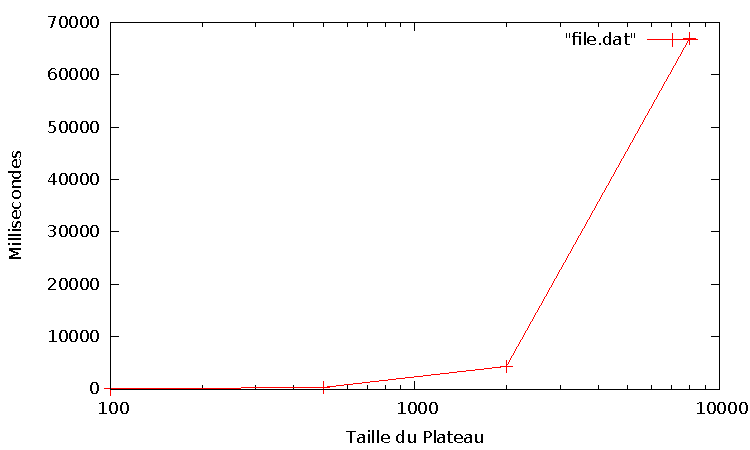
\includegraphics[scale=0.5]{pthread.pdf}
	\end{center}
	\caption{Exécution avec Pthread \label{fig:life_pthread}}
\end{figure}

\section{Version mémoire distribuée}
\subsection{mpi avec communications synchrones}
\paragraph{} Dans cette version, un process MPI va initialiser la grille, on met en place un communicateur cartésien sur les process et on utilise un scaterv() pour pouvoir répartir la grille entre les différents process.

\paragraph{}Chaque process détient donc un morceau de la grille, il va donc falloir récupérer dans un premier temps, avec des communications synchrones, les cellules voisines de cette grille sur les autres process avant de pouvoir compter le nombre de voisins et mettre à jour les cellules. Un gatherv est utilisé pour rassembler la grille à la fin.

\paragraph{}On remarque que cette version est moins performante que la version pthread et cela s'explique par le fait que les communications sont synchrones. En effet, chaque process doit attendre de posséder toutes ses cellules voisines avant de pouvoir commencer les calculs.

\paragraph{}Les tests ont été effectués avec 9 process mpi pour des tailles de grille de 9, 90, 450, 1800, 7200. (la taille devant être divisible par le nombre de process étant lui même une puissance).

\begin{figure}[!h]
	\begin{center}
		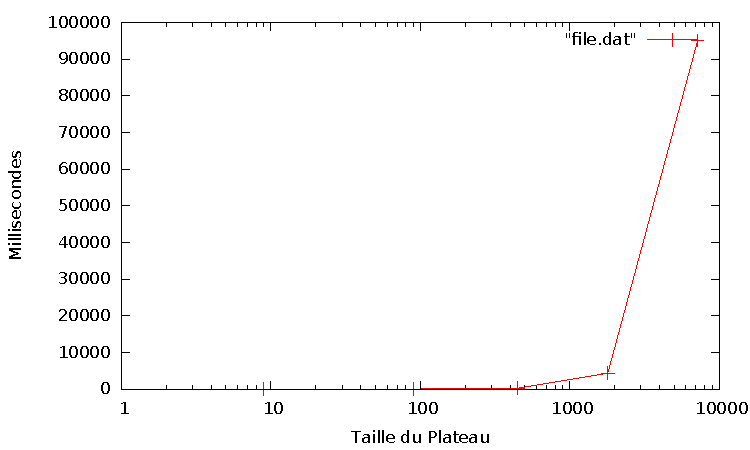
\includegraphics[scale=0.5]{mpi_synch.pdf}
	\end{center}
	\caption{Exécution MPI avec communications synchrones \label{fig:life_mpi_synch}}
\end{figure}

\subsection{mpi avec communications asynchrones}
\paragraph{}Malheureusement nous n'avons pas mener à terme cette section, mais l'idée est de rendre les communications asynchrones pour pouvoir commencer les calculs sans attendre la fin des communications.

\paragraph{}On veut toujours recevoir, les cellules voisines des bords de la sous-grille, on initie donc les communications permettant de les récupérer mais même si les communication ne sont pas terminées on peut commencer à calculer les voisins des cellules "intérieurs", c'est à dire celles qui ont toutes des cellules voisines locales. On gagne ainsi du temps car les communications sont recouvertes par le calcul.

\end{document}